%%%%%%%%%%%%%%%%%%%%%%%%%%%%%%%%%%%%%%%%%%%%%%%%%%%%%%%%%%%%%%%%%%%%%%%%%%%%%%%%
%% Aalaadin/AGR                                                               %%
%%%%%%%%%%%%%%%%%%%%%%%%%%%%%%%%%%%%%%%%%%%%%%%%%%%%%%%%%%%%%%%%%%%%%%%%%%%%%%%%
\section{Aalaadin/AGR}

% Aallaadin/AGR - references
This section introduces the Aalaadin/AGR\footnote{`Aalaadin' is the old name, whereas `AGR' is the new one. Since it is arguably fancier, we will use the old name.} metamodel described in \cite{Ferber97}, \cite{Ferber98}, \cite{Ferber00} and \cite{Ferber03}.
The overview presented here is particularly after \cite{Ferber98}.

% Aalaadin/AGR - authors
Aalaadin/AGR has been proposed in 1997 by Jacques Ferber, Oliver Gutknecht and their colleagues from Montpellier 2 University in Montpellier, France.

%% Summary %%%%%%%%%%%%%%%%%%%%%%%%%%%%%%%%%%%%%%%%%%%%%%%%%%%%%%%%%%%%%%%%%%%%%

- PIM

% Aalaadin - about
Aalaadin is a platform-independent (ALT: generic) metamodel of multiagent systems based on three core concepts: agent, group and role.
It is actually what its authors refer to as \textit{organization-centric multiagent system} (OCMAS) metamodel, because it enables a MAS designer to build/describe/specify various organization models such as flat (e.g. market-like) or hierarchical (e.g. enterprise-like) organizations.

In the following subsections, the Aalaadin metamodel (called simply model) will be introduced.
The model itself has two levels:
\begin{itemize}
	\item The \textbf{concrete level} contains relatively concrete concepts like \textit{agent}, \textit{group} and \textit{role}.
	The language defined by this level is used to describe concrete organizations.
	\item The \textbf{abstract level} contains more abstract concepts like \textit{group structure}, \textit{organization structure} and \textit{interaction}. 
	The language of this level is used to describe abstract organizations, i.e. families of organizations sharing the same structural characteristics.
\end{itemize}

% TODO Concrete organization vs. abstract organization
To understand the following text, it is essential to make a distinction between a \textit{concrete organization} and \textit{abstract organization}.
A concrete organization is the actual organization that exists in a MAS at run-time, whereas an abstract organization is the organization specification that exists in a MAS at design-time.
To put it differently, an abstract organization represents a (possibly infinite) set of all imaginable organizations conforming to common specification and a concrete organization represents a member of this set.

% Organization instance vs organization class
Later we will use the terms \textit{organization instance} and \textit{organization class} to refer to an concrete organization and abstract organization respectively.
These terms try to capture the essence of the relationship between an abstract and concrete organization (namely, a concrete organization being an instance of an abstract organization and conversely, an abstract organization being a class of a concrete organization) and are imported from OOP where it is necessary to make a similar distinction. 

%%%%%%%%%%%%%%%%%%%%%%%%%%%%%%%%%%%%%%%%%%%%%%%%%%%%%%%%%%%%%%%%%%%%%%%%%%%%%%%%
\subsection{Core Concepts}

% Core model - about
The Aalaadin core model is based on three \textit{core concepts}: \textit{agent}, \textit{group} and \textit{role}.
Figure~\ref{figure:aalaadin-core-model} shows a diagram of the core model.

% Figure: Aalaadin core model
\begin{figure}[h]
	\centering
	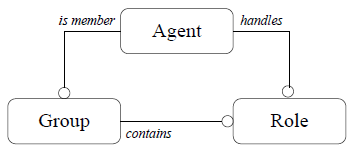
\includegraphics[width=0.5\textwidth]{images/aalaadin-core-model.png}
	\caption{The Aalaadin core model}
	\label{figure:aalaadin-core-model}
\end{figure}

\subsubsection*{Agent}

% Agent - definition
An \textit{agent} is defined in \cite{Ferber97} as an active communicating entity which plays \textit{roles} within \textit{groups}.

% Agent - no agent architecture imposed
The Aalaadin model does not prescribe any particular agent architecture.
Any metamodel striving for generality should impose as little constraints upon the MAS designer as possible.
After all, the decision of which agent architecture to use is best made by the designers themselves and relates to the MAS as such, not just its organizational structure.
As we will see, none of the metamodels introduced in this thesis force the MAS designers to adapt a concrete definition of agenthood.

\subsubsection*{Group}

% Group - definition
In \cite{Ferber97}, \textit{groups} are defined as atomic sets of agent aggregation.
Each agent belongs to one (possibly none) or more groups.

% Group - about
In its most basic form, a group is just a way to tag a set of agents, i.e. it has no structure.
The real advantage of grouping agents becomes apparent when we introduce some order \footnote{The casual, not formal, meaning of the word is intended here.} to these groups.
This order can be achieved using roles.

% Group - characteristics
Groups have the following characteristics:
\begin{itemize}
	\item An agent can be a member of any number of groups simultaneously.
	This means that group can overlap, which is major point of Aalaadin.
	\item A new group can be founded by any agent and an agent must request its admission to an existing group.
	\item A group may be local or distributed across multiple machines.
\end{itemize}

\subsubsection*{Role}

% Role - definition
A \textit{role} is an abstract representation of n agent function, service or identification within a group \cite{Ferber97}.
An agent can play multiple roles each of which is local to a group.
Similarly to group admission, playing a group in a role must be requested by the candidate agent (already belonging to the group) and awarded by the founder agent.

% Role & communication
In Aalaadin, the communication is related to roles. Since an agent can play multiple roles, the model allows it to engage in multiple independent dialogs simultaneously.

% Role - definition characteristics
The following characteristics are part of a role definition:
\begin{itemize}
	\item \textit{uniqueness}. A role can be \textit{unique} or \textit{multiple} within a group.
	A unique role can be played by at most one agent in a given group.
	A multiple role, on the other hand, can be played by any number of agents in a given group. 
	\item a list of competences. A \textit{competence} specifies a condition the candidate agent must satisfy to be eligible to play the role within the group. 
	\item a list of capacities. A \textit{capacity} specifies an ability attributed to an agent while it is playing the role.
\end{itemize}
By default a role is multiple, does not require any competences and does not provide any capacities.

% Group manager role
A special role in a group is the \textit{group manager} role, which is automatically granted to the group founder.
It has a competence to handle group membership and role playing requests.
It also has a capacity to revoke roles and cancel group memberships.

%%%%%%%%%%%%%%%%%%%%%%%%%%%%%%%%%%%%%%%%%%%%%%%%%%%%%%%%%%%%%%%%%%%%%%%%%%%%%%%%
\subsection{Methodological Concepts}

% Methodological model - about
The Aalaadin methodological model contains so-called \textit{methodological concepts}.
These concepts are not present directly in concrete organizations but only serve during the analysis and design phases.
Their purpose is to describe an abstract organization from which the concrete organization will ultimately be derived and described using the core concepts.
Figure~\ref{figure:aalaadin-metamodel} presents the entire Aalaadin metamodel. The core model is demarcated with dotted ellipsis.

% Figure: Aalaadin metamodel
\begin{figure}[h]
	\centering
	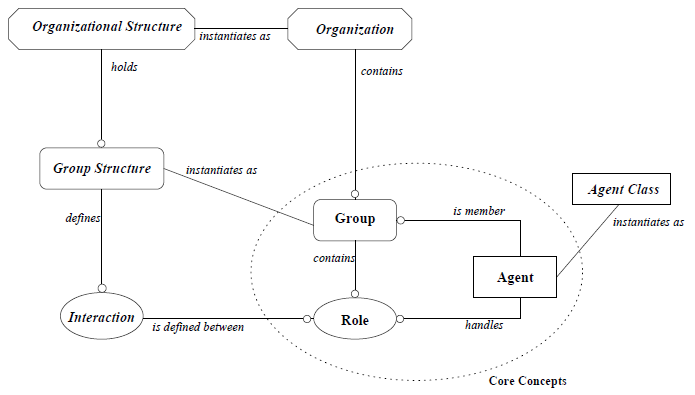
\includegraphics[width=0.75\textwidth]{images/aalaadin-metamodel.png}
	\caption{The Aalaadin metamodel}
	\label{figure:aalaadin-metamodel}
\end{figure}

\subsubsection*{Group Structure}

% Group structure - definition
A \textit{group structure} is an abstract description of a group \cite{Ferber97}.
It identifies all roles comprising the group and defines interactions among them.

% Group structure - definition characteristics
A group structure is defined by:
\begin{itemize}
	\item a list of available roles (see role definition) that can be played by agents in the group,
	\item a set of valid interaction schemes (including language) among roles.
\end{itemize}

% Group structure - partial instantiation
Note that a group might be a partial instantiation of its defining group structure.
This means that some roles defined in the group structure might not be played at the moment in the group.
This dynamic nature of groups allows for a great deal of run-time flexibility.
Contrast this with plain vanilla MAS where an agent, once an instance of a particular agent class, can not change this class at run-time.

\subsubsection*{Organizational Structure}

% Organizational structure - definition
The \textit{organizational structure}, as defined in \cite{Ferber97}, is a set of group structures expressing the design of a multiagent organization scheme.

% Organizational structure - about
The organizational structure can be seen as the specification of the problem to be solved (organization to be modelled) using a MAS.
Any sort of heterogeneity within a single system (e.g. agent architecture or language heterogeneity) can be managed by different group structures involved in the organizational structure.

% Organizational structure - partial instantiation
Similarly to groups, the actual organization is just one possible manifestation of the organizational structure.
Some groups defined in the organizational structure might not be present currently in the organization.
This also contributes to the overall run-time flexibility.

%%%%%%%%%%%%%%%%%%%%%%%%%%%%%%%%%%%%%%%%%%%%%%%%%%%%%%%%%%%%%%%%%%%%%%%%%%%%%%%%
\subsection{MadKit}

% MadKit - authors & references
The authors of Aalaadin/AGR also developed what started out as a proof-of-concept agent platform called \textbf{MadKit} (Multi-Agent Development Kit).
It has been described in an (unpublished) research report \cite{Ferber97} and a conference/workshop articles \cite{Ferber98} and \cite{Gutknecht00}.

%MadKit - design principles
The \textbf{MadKit} platform implements the Aalaadin/AGR core model and follows three design principles \cite{Ferber97}:
\begin{itemize}
	\item micro-kernel architecture,
	\item agentification of services and
	\item graphic component model.
\end{itemize}

% MadKit - basic philosophy
The basic philosophy of the Aalaadin/MadKit architecture is to use the platform itself for its own management wherever possible.
All services except for the most fundamental ones provided by the micro-kernel are implemented as agents, organized in groups and identified by roles \cite{Ferber98}.

% MadKit - technical details and requirements
\textbf{MadKit} is written in the Java programming language and runs on the Java platform, version 1.1.